\documentclass[pdf]{beamer} % Add the [handout] option to group all of the items
\usetheme{Copenhagen}

\usepackage{pgfpages}
%\setbeameroption{show notes on second screen=right}
%\setbeameroption{show only notes}
\usepackage[utf8]{inputenc}
\usepackage[spanish]{babel}
\usepackage{paralist}
\usepackage{stmaryrd}
\usepackage{graphicx,xcolor}
\usepackage{subcaption}
\usepackage{array}
\usepackage{color}




\title{Formalización del sistema de permisos de Android 10}

\author[Universidad Nacional de Rosario]{Guido De Luca}
\institute{Universidad Nacional de Rosario}
\date{\today}

\subject{Tesina}


\begin{document}

\begin{frame}[plain]
    \titlepage
\end{frame}

\begin{frame}{Motivación}
    \begin{itemize}
        \item ¿Por qué Android? \pause Por su popularidad y alcance \pause
        \item ¿Por qué un sistema de permisos? \pause Mediador entre usuarios y aplicaciones \pause
        \item ¿Por qué métodos formales? \pause
              \begin{itemize}[<+->]
                  \item Pruebas rigurosas
                  \item Aclarar comportamientos ambiguos
                  \item Construir un framework para razonar sobre el sistema
              \end{itemize}
    \end{itemize}
\end{frame}

\begin{frame}{J.P. Anderson, 1972}
    Diseño de un mecanismo de validación por referencia:
    \pause
    \begin{itemize}[<+->]
        \item Mediación completa
        \item A prueba de manipulaciones
        \item Verificable
    \end{itemize}

    \begin{block}{Definición}
        % +1 por el \pause del principio
        \only<2>{Toda acción ejecutada por el sistema debe ser supervisada por el monitor de
            referencia.}

        \only<3>{ La ejecución del MVR no debe ser modificable manual ni programáticamente. Más
            conocido en ingles como \textit{tamper-proof}.}

        \only<4>{La implementación del validador de referencia debe ser lo suficientemente pequeña
            para ser verificable y \textit{testeable} de manera exhaustiva.}
    \end{block}
\end{frame}

\begin{frame}{Un poco de contexto sobre Android}
    \begin{columns}
        \begin{column}{.6\textwidth}
            \textbf{Arquitectura de pila:} \pause
            \begin{enumerate}[<+->]
                \item Aplicaciones del sistema y de terceros
                \item \textit{API} de la plataforma
                \item Entorno de \textit{runtime} y bibliotecas nativas
                \item Capa de abstracción del hardware
                \item Núcleo de Linux
            \end{enumerate}
        \end{column}

        \begin{column}{.4\textwidth}
            \begin{figure}
                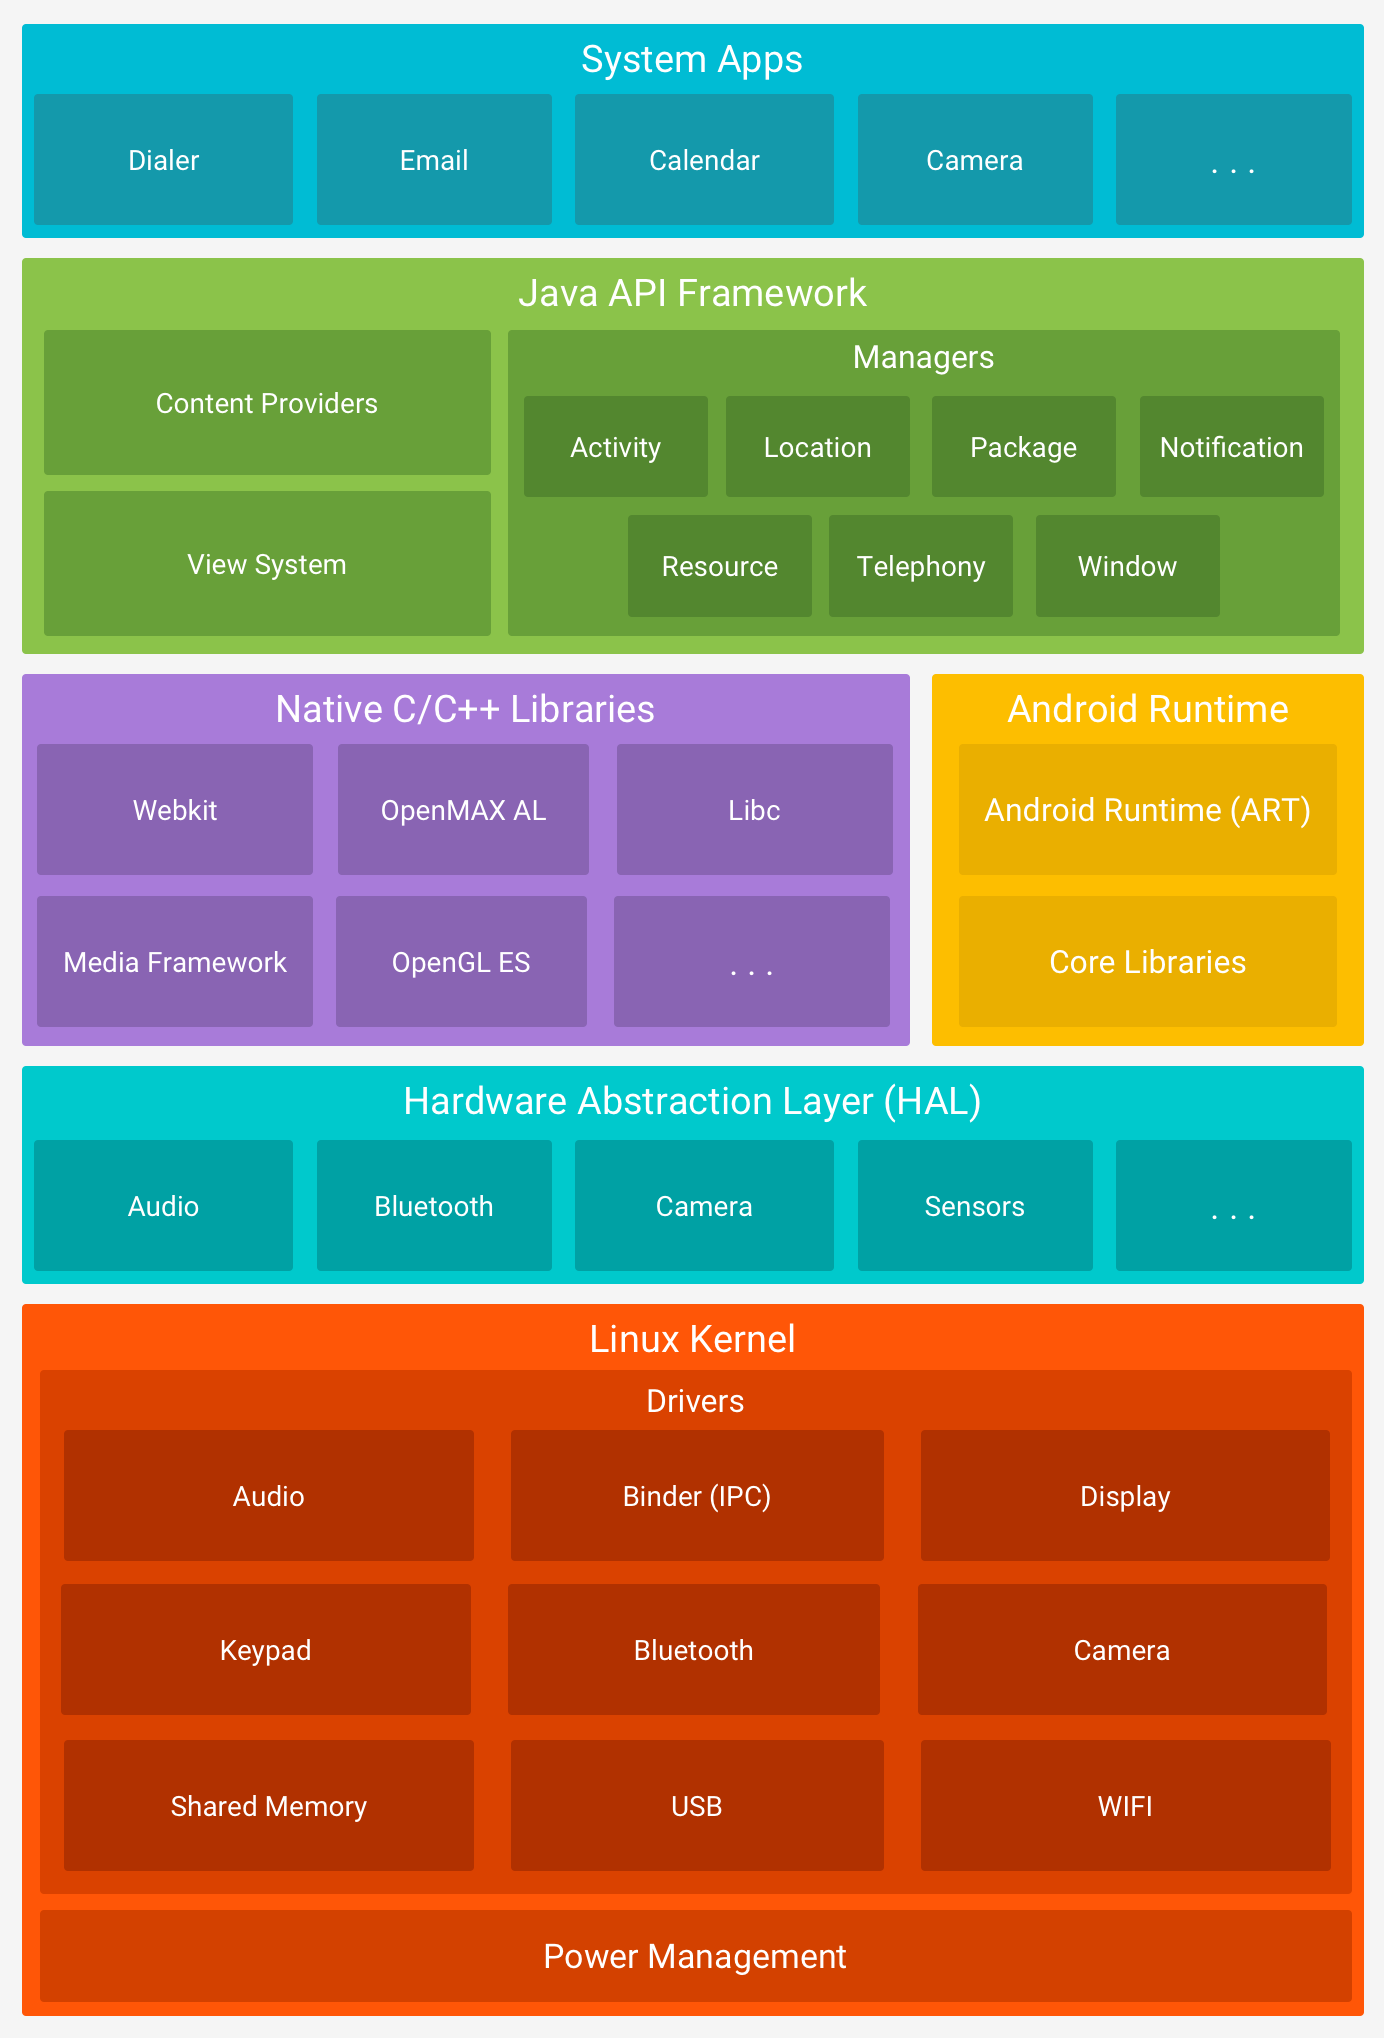
\includegraphics[scale=0.1]{../imagenes/android-stack.png}
            \end{figure}
        \end{column}
    \end{columns}


\end{frame}

\end{document}